%%%%%% Krav %%%%%%
\chapter{Krav}
\vspace{-0.5cm}
I dette afsnit beskrives kravene til projektet [1]. Indledningsvis præsenteres funktionelle krav  ved brug af use cases. På figur \ref{fig:useCaseDiagram} vises et use diagram, der viser aktører og use cases tilhørende systemet. Efter use case diagrammet følger en kort beskrivelse af de seks use cases og deres funktion. Afsnittet afsluttets med ikke-funktionelle krav, der både er krav til systemet som helhed og til systemets blokke.
\vspace{-0.3cm}

\section{Funktionelle krav}
\vspace{-0.2cm}
Til systemet er der identificeret de 2 aktører: Bruger \& GPS-satellitter. Bruger er primær aktør der ønsker at initialisere og styre systemet. Bruger er ansvarlig for at oprette flyveopsætninger på webapplikationen og tilslutte batteri til dronen.
GPS-satellitter er sekundær aktør, der gør det muligt for dronen at finde egen position. 
På figur \ref{fig:useCaseDiagram} vises et use case diagram, der viser systemets aktører og i hvilke use cases aktørerne optræder. 
\begin{figure}[H]
	\centering
	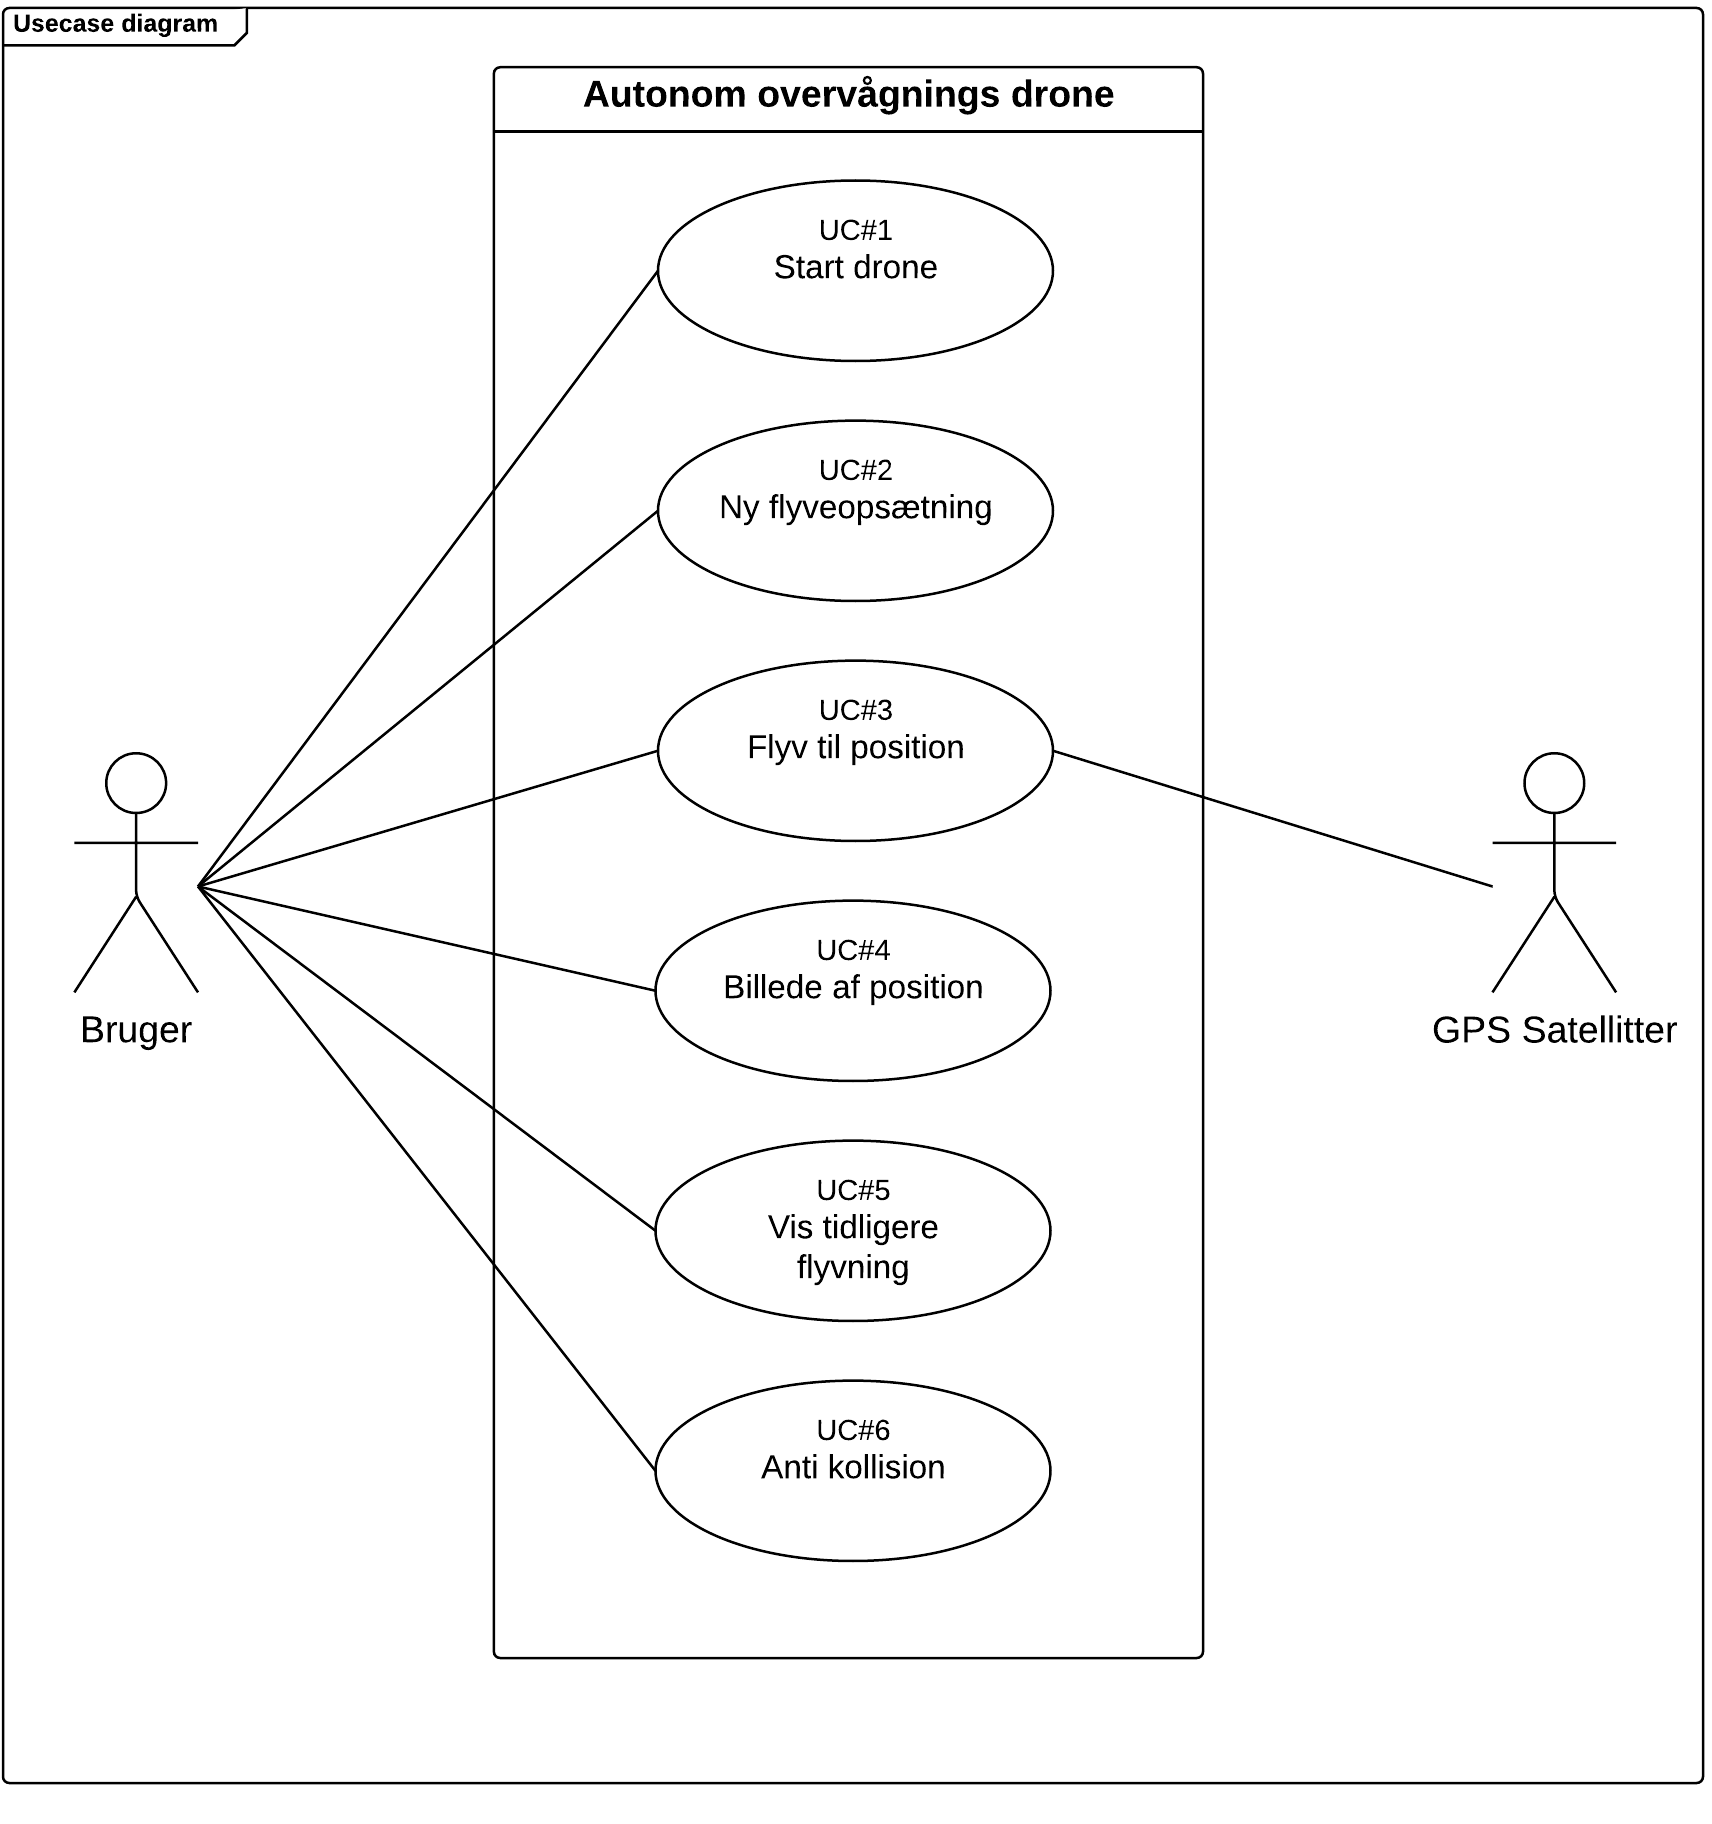
\includegraphics[width=0.75\textwidth]{Billeder/Krav/Use_case_diagram}
	\vspace{-0.3cm}	
	\caption{Use case diagram}
	\label{fig:useCaseDiagram}
\end{figure}

\newpage

I projektets kravspecifikation er alle use cases beskrevet som fully dressed use cases. I fully dressed use cases beskrives hvordan hovedforløb ser ud i en given use case, hvis den succesfuldt gennemføres. Desuden beskrives startbetingelse, aktører og tilføjelser.

Nedenfor beskrives hovedforløb og funktion af de seks use cases:\\

\textbf{Use case 1: Start drone} \\
Bruger tilslutter batteri til drone og dronen initialiseres. Drone sender information om nuværende position til server.\\

\textbf{Use case 2: Ny flyveopsætning} \\
Bruger logger på webapplikation og opretter en ny flyveopsætning. Flyveopsætningen sættes tilgængelig for drone på server.\\

\textbf{Use case 3: Flyv til position}\\
Drone henter flyveopsætning fra server og påbegynder flyvning. Under flyvning tilpasser drone  løbende flyvehøjde og flyveorientering og fortsætter flyvning mod ønsket position. \\

\textbf{Use case 4: Billede af position} \\
Når drone er ankommet til ønsket GPS position tages et billede. Hvis billedet accepteres, flyver dronen videre mod næste GPS koordinat eller til udgangsposition. \\

\textbf{Use case 5: Vis tidligere flyvninger} \\
Bruger tilgår webapplikation for at se flyveruter og billeder fra tidligere flyvninger.\\

\textbf{Use case 6: Antikollision} \\
Drones antikollisionssensorer bruges til at detektere forhindringer. I tilfælde af forhindringer ændrer dronen enten flyveretning eller flyvehøjde for at undgå kollision. \\



\section{Ikke-funktionelle krav}

De ikke-funktionelle krav opstilles ud fra systemspecifikationerne og er krav som ikke kan defineres i use cases. Disse krav har ingen indvirkning på systemets endelige funktion, kun systemspecifikationer.  

De ikke-funktionelle krav opstilles i fem grupper. Nogle krav er generelle krav til systemet, mens andre krav mere specifikt omhandler drone, server og webapplikation eller dataopsamling. 
De ikke-funktionelle krav bruges til at sikre system performance, eksempelvis stilles krav til de hardwaremoduler og sensorer der er monteret på dronen. 
